
\documentclass{include/thesisclass3}

\SelectLanguage{english}
\usepackage{float}


% Titlepage settings
\newcommand{\praktikum}{Praktikum moderne Physik}
\newcommand{\autora}{Jens Schäfer}
\newcommand{\autorb}{Jan van der Linden}
\newcommand{\maila}{ugecd@student.kit.edu}
\newcommand{\mailb}{jan.vdlinden95@gmail.com}
\newcommand{\topic}{Landé factor of the muon}
\newcommand{\ptime}{12. Juni 2017}


% Shortcuts
\newcommand{\cc}{\cdot}
\newcommand{\rk}{\rangle}
\newcommand{\lk}{\langle}
\newcommand{\df}{\rightarrow}
\newcommand{\la}{\lambda}
\newcommand{\dd}{{\rm d}}
\newcommand{\ehm}{\mathbbm{1}}
\newcommand{\p}{\partial}
\newcommand{\soll}{\overset{!}{=}}
\newcommand{\D}{\Delta}
\newcommand{\eps}{\epsilon}
\newcommand{\vektor}[3]{\begin{pmatrix} #1 \\ #2 \\ #3 \end{pmatrix}}
\newcommand{\vektorz}[2]{\begin{pmatrix} #1 \\ #2 \end{pmatrix}}
\newcommand{\Mat}[9]{\begin{pmatrix}#1&#2&#3\\#4&#5&#6\\#7&#8&#9\end{pmatrix}}
\newcommand{\Matz}[4]{\begin{pmatrix}#1&#2\\#3&#4\end{pmatrix}}
\newcommand{\e}[1]{\,\si{#1}}
 


\begin{document}

	\FrontMatter
	% coordinates for background border
\newcommand{\diameter}{20}
\newcommand{\xone}{-15}
\newcommand{\xtwo}{160}
\newcommand{\yone}{15}
\newcommand{\ytwo}{-253}




\begin{titlepage}
    % background border
    \begin{tikzpicture}[overlay]
    \draw[color=gray]
            (\xone mm, \yone mm)
      -- (\xtwo mm, \yone mm)
    arc (90:0:\diameter pt)
      -- (\xtwo mm + \diameter pt , \ytwo mm)
        -- (\xone mm + \diameter pt , \ytwo mm)
    arc (270:180:\diameter pt)
        -- (\xone mm, \yone mm);
    \end{tikzpicture}



    % KIT image and sign for faculty of physics
    \begin{textblock}{10}[0,0](4.5,2.5)
        
\includegraphics[width=.25\textwidth]{include/kitlogo.pdf}
    \end{textblock}
    

    % horizontal line
    \begin{textblock}{10}[0,0](4.2,3.1)
        \begin{tikzpicture}[overlay]
        \draw[color=gray]
                (\xone mm + 5 mm, -12 mm)
          -- (\xtwo mm + \diameter pt - 5 mm, -12 mm);
        \end{tikzpicture}
    \end{textblock}



    % begin of text part
    \changefont{phv}{m}{n}    % helvetica
    \centering



    % thesis topic (en and ge)
    \vspace*{3cm}
    \Huge\praktikum\\



    % author name and institute
    \vspace*{5cm}
    
    \huge\topic\\






    % examiners (Referenten)
    \vspace*{3cm}
    \Large
    \begin{center}
        \begin{tabular}[ht]{l c l } 
  \autora & \hfill & \textit{\maila} \\
\autorb & \hfill & \textit{\mailb} \\
        
        \end{tabular}
    \end{center}



    % working time
    \vspace{2cm}
    \begin{center}
        \large{Durchgeführt am}: \ptime
    \end{center}



    % lowest text blocks concerning the KIT
    \begin{textblock}{10}[0,0](4,16.8)
        \tiny{KIT -- Universität des Landes Baden-Württemberg und nationales %
              Forschungszentrum in der Helmholtz-Gemeinschaft}
    \end{textblock}
    \begin{textblock}{10}[0,0](14,16.75)
        \large{\textbf{www.kit.edu}}
    \end{textblock}
\end{titlepage}

	\tableofcontents                  
	\newpage
	\MainMatter

%Protokollstart

\chapter{Theoretical Background}

In this experiment the lifetime of a muon is to be determined, as well as its Landé factor.
For this, a coincidence trigger will be used, measuring the time difference between a muon coming into the apparatus and the decay particle, a positron being detected.

\section{Cosmic muons}
Primary cosmic radiation consists mainly of protons (85\%), alpha particles and photons.
When entering the atmosphere secondary particles are induced by interacting with the matter in the atmoshpere.
A strong interaction with air molecules induces the production of pions, protons and neutrons.
Due to the short halflife of pions, they do not reach the earth, but rather convert either into a pair of photons (in the case of the neutral pion) or into a charged lepton and its corresponding anti-neutrino ($\pi^\pm ~\df~ \mu^\pm + \nu_\mu/\bar{\nu}_\mu$).
The produced muons have a higher range in comparison with the electrons, because they are far heavier.
Also, due to the high energies of the cosmic radiation, also the muons have very high energies and are therefore ultrarelativistic.
As the mean lifetime of a muon is approximately $\tau = 2.2\cc10^{-6}\e{s}$ they should in gerneral not be able to reach earth.
The muons are however ultrarelativistic, which enables them to reach earth, because the lifetime is calculated for the restframe of the muon, which translates to $\tau_E = \gamma \tau$ in an observers frame.
Therefore even muons with energies of $10\e{GeV}$ are able to travel over $60\e{km}$ or more.

In matter, high energy muons lose energy mainly by bremsstrahlung; the emission of photons.
In lower energy ranges (under GeV) they also lose notable amounts of energy from ionization processes or coulomb interaction.
Furthermore, negative muons $\mu^-$ get caught by atoms and get absorbed into the nucleus by interacting via the weak force.
Thus, the lifetime of $\mu^-$ reduces a lot when passing through matter, which results in the main part of the cosmic muon radiation to consist of positive muons $\mu^+$.

At the end of the lifetime of the positive muons they usually convert into positrons via $\mu^+ ~\df~e^+ + \mu_e + \bar{\nu}_\mu$. 
\section{Muon polarization}
%In certain energy intervals, the momentum of muons is polarized, because of the parity violation of the weak interaction.
As pions carry spin $0$ and it decay particle the neutrino must have negative chirality due to its velocity (or its vanishing mass) the antimuon is forced by conservation of spin and momentum to have negative chirality aswell (maximum parity violation of weak interaction only permits particles of negative and antiparticles of possitive chirality).
Now, the muons also have different energies, depending on the direction of emission from the pion.
If the muon is emitted in the direction of travel in the rest frame of the decaying pion, it has a higher energy than the muons emitted in the opposite direction. For a muon emitted against the direction of travel, a negative polarization is expected, whereas a positive polarization is expected for the muons emitted in the direction of travel.
Observing a certain energy interval there are muons with equal energys but different polarization depending on if it was emitted by low-energy pions in direction of travel or by high-energy pions in the opposite direction. As a matter of fact there is a non-equal distribution of pions in different energy scales. Thus, there will be a polarization of approximately $P=-\frac{1}{3}$ observable, if an energy sensitive measurement will be performed at an angle purpendicular to the sincidence angle.

\section{Evidence of muon decay}
To measure a decaying muon the conversion into a positron $e^+$ and two invisible neutrinos has to be observed.
The double differential cross section for this process is given by
$ \frac{\d N}{\d \eps \d \Omega} = \frac{\eps}{2\pi} \left[ (3-2\eps) - P(1-2\eps)\cos\theta\right] \equiv a(1 + b \cos\theta) $
Here, $\eps$ denotes the relative energy $\eps = E/E_{max}$, where $E_{max} = m_\mu/2$, and $\theta$ denotes the angle between the spin of the incident muon and the momentum of the positron. 
The polarization of the muon is called $P$.

\section{Landé factor of the muon}
With a magnetic field applied, the muon precesses around the direction of $B$ with frequency $\omega = \gamma B$ where $\gamma$ is the gyromagnetic ratio
\[ \gamma = g \frac{\mu_B}{\hbar}, ~~~\mu_B = \frac{e\hbar}{2m}\]
For the muon, the Bohr magneton is equivalent to $\mu_B = 4.5\cc10^{-26}\e{\frac{J}{T}}$ and $g$ is the Landé factor of the muon.
This factor can be measured through measurement of the precession frequency of a free particle in a magnetic field, such that
\begin{equation} g = \frac{\hbar \omega}{\mu_B B}
\label{lande}
\end{equation}

\section{Principle of measurement}
By observing the time difference between the muon decellerating in the detector and the appearence of the positron the mean lifetime can be calculated by histogramming the time differences. The shape of the histogrammed events is expected to follow the distribution of an exponential decay.
\begin{equation}
N(t)=N_0\,e^{-t/\tau}
\end{equation}
For the detection, three szintillators are layered with a copper absorber inbetween the last two layers. Each layer is about $2.5\e{cm}$ thick. With trigger hardware only muons passing through layer 1 and 2 but not through 3 are counted. 
For the Landé factor the precession frequency has to be measuered. For this, the mean lifetime gets observed but just on a decent angle $\theta$. The ratio of decaying myons is now modulated by the precession and the angle is time dependant with $\theta = \omega t$, so the mean lifetime goes to 
\begin{equation}
N(t)=K\cdot e^{ -t/\tau } \cdot [ 1+\bar A \cdot \cos(\omega t + \delta )]\label{n(t)}
\end{equation}

\chapter{Analysis}
Due to the low event rate in the used detector, a dataset gathered in the last two years was used. 
This data set consists of over 200000 events assumed to be lifetime signatures of the muons.
\section{Time calibration}
As the detector is categorizing the time differences in terms of channels firstly a time calibration had to be done.
The result is show in figure \ref{time}.

\begin{figure}[H]
\centering
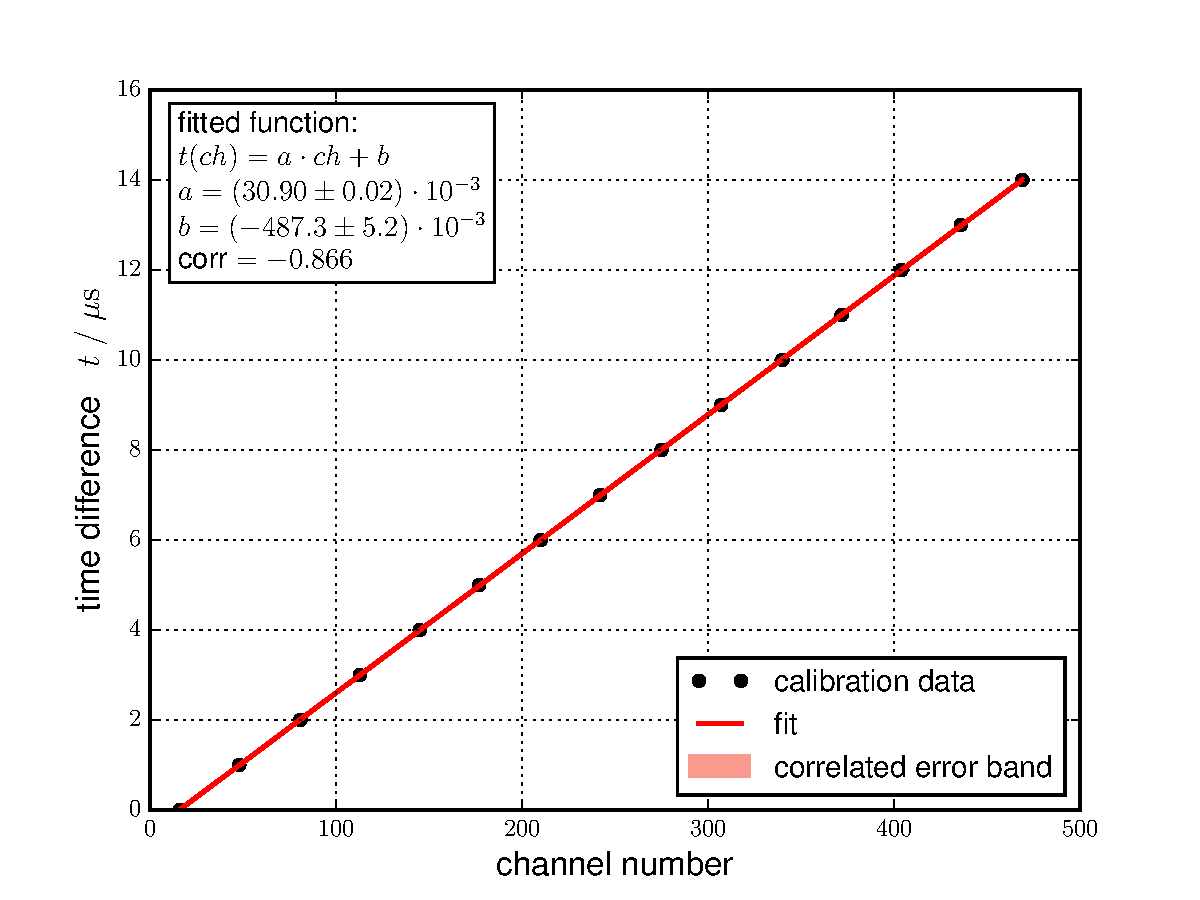
\includegraphics[width = 0.8\textwidth]{images/cali_fit.pdf}
\caption{\label{time}\textbf{Time calibration.} To calibrate the channel numbers to the measured time differences an artificial time delay of $1\e{\mu s}$ to $20\e{\mu s}$ in steps of $1\e{\mu s}$ were introduced in the wiring. The active channel was then recorded and used for the calibration. The resulting calibration is then given by the linear fit.}
\end{figure}
The data then was linearly rescaled with following function which rescales the channel number $ch$ to a time difference $t(ch)$
\[ t(ch) = (30.90 \pm 0.02)\cc 10^{-3} \e{\mu s} \cc ch - ( 487 \pm 5) \cc 10^{-3} \e{\mu s}\]
The resulting data with errors is shown in figure \ref{raw}. The errors in time were calculated with gaussian error propagation through the errors in the time calibration. The errors in the number of registered muons $N$ was assumed to be poisson distributed with an uncernaity of $\sqrt{N}$.

\begin{figure}[H]
	\begin{center}
		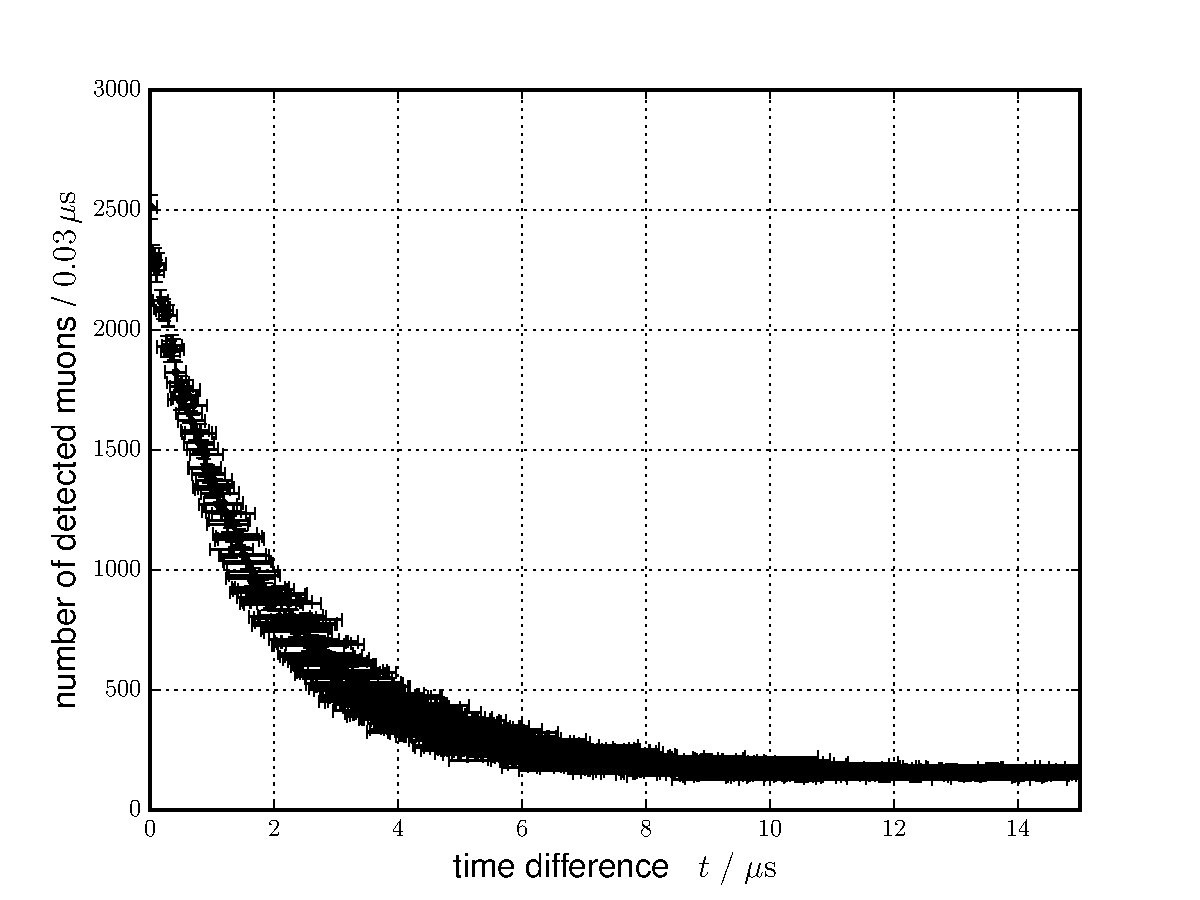
\includegraphics[width=0.75\textwidth]{images/errors.pdf}
		\caption{\label{raw}\textbf{Rescaled data with errors.} Shown is the rescaled data with the number of detected muon events over the measured time differences corresponding to the muon lifetimes. To increase the readability of following plots, the errorsbars are only shown in this figure.}
	\end{center}
\end{figure}
The data should follow a distribution as given in equation \ref{n(t)} plus a constant background. 
To fit this function it is possible to fit all six parameters at once to the data (section \ref{first}) or to split the data into two sets where the first set for smaller times behaves exponential and the second one linear (section \ref{second}). By fitting each section on its own the separated parameters can be fitted more precise. 
\section{First method: six parameter fit}
\label{first}
The data recorded in figure \ref{raw} describes an exponential decay of the muon with lifetime $\tau$ modulated with an osscilating term from the precession of the muon spin with frequency $\omega$. 
With the constant background $C$, the scaling of the exponential $K$, the scaling of the oscillation $\bar A$ and its phase $\delta$ these six parameters were fitted simultaneously onto the set of data. The results are shown in figure \ref{6pm}.
\begin{figure}[H]
\centering
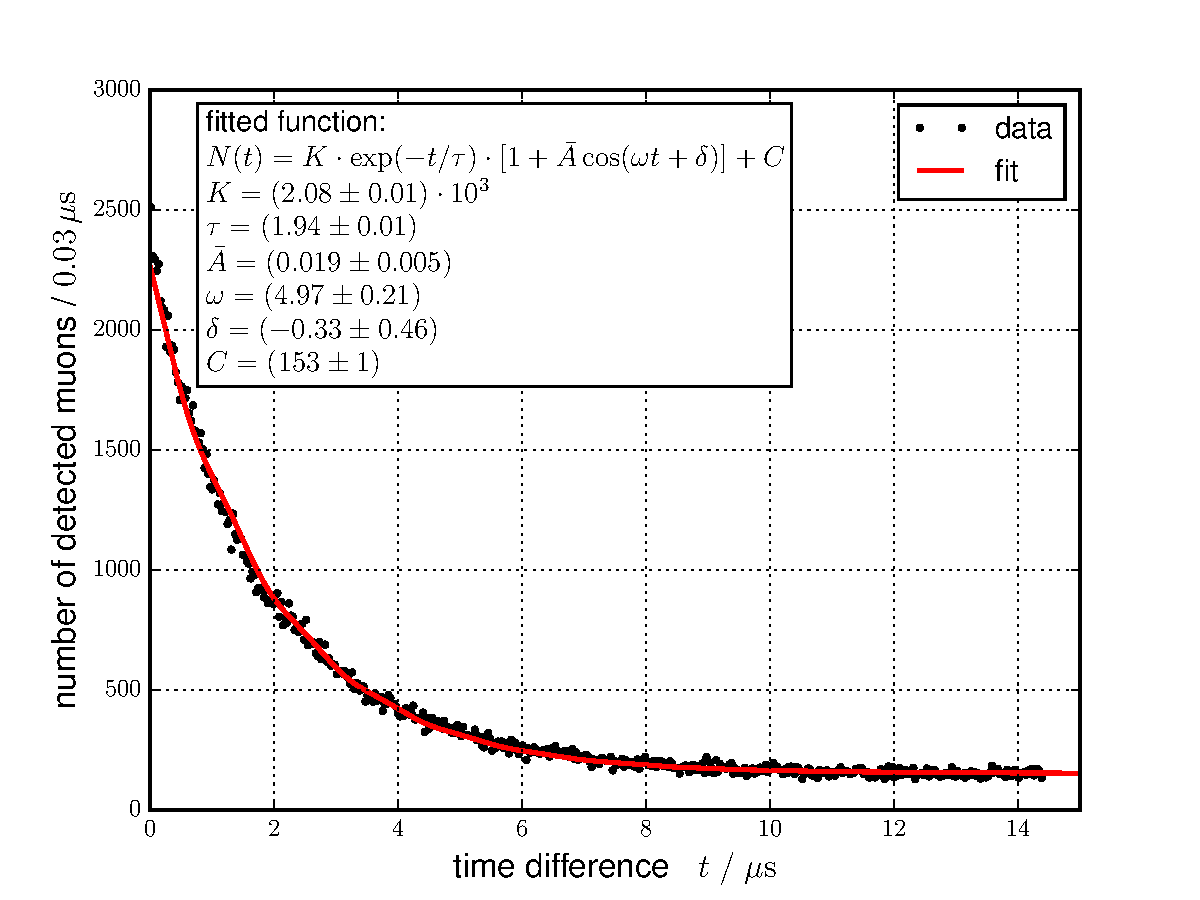
\includegraphics[width= 0.8 \textwidth]{images/6paramfit.pdf}
\caption{\label{6pm}\textbf{Six parameter fit.} For this fit all six parameters were fitted simultaneously. Errors both in time and number were regarded in this fit.}
\end{figure}
The resulting lifetime of the muon can directly be read off the fit as the parameter $\tau$. 
The Landé factor first has to be calculated with equation \ref{lande} from $\omega$.
The uncernaity was propagated from $\omega$ to $g$ with gaussian error propagation.
\begin{align}
&\e{Lifetime} &\tau &=(1.94\pm 0.01)\e{\mu s}\\
&\e{Landé~factor} &g &=3.2 \pm 0.1
\end{align}


\section{Second method: separate fits}
\label{second}
\begin{figure}[H]
	\begin{center}
		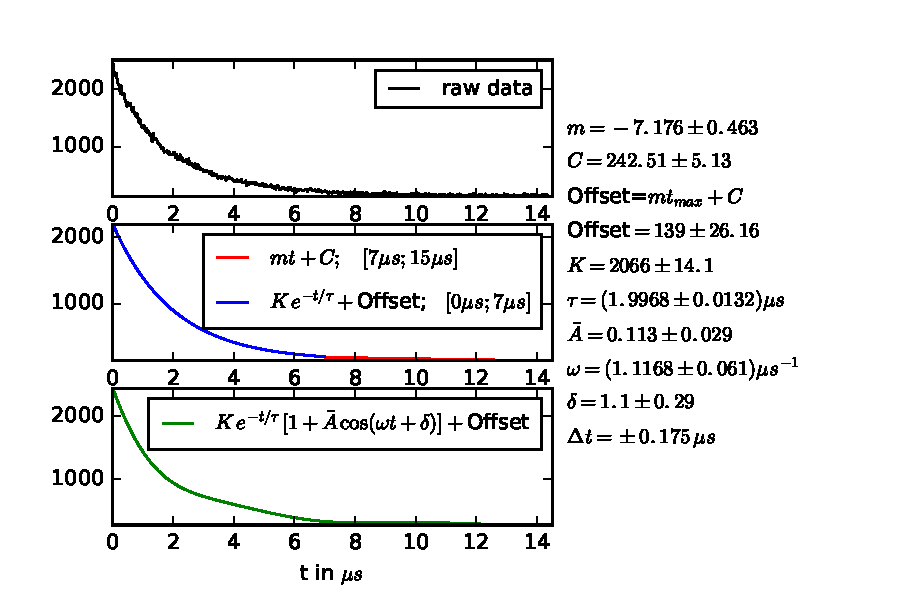
\includegraphics[width=0.8\textwidth]{images/plot.pdf}
		\caption{Raw data and three fits via the second methond are displayed aswell as the fitted functions and parameters}
		\label{method2}
	\end{center}
\end{figure}
The division took place after 7$\e{\mu s}$. The second area gives a linear function, its lowest point is interpreted as the background noie. This offset will be added on the next two fits. With knowledge of this offset the next fit in exponential shape could be done. Therefore the first area is used and the parameters K and $\e{\tau}$ were calculated. After these two fits shown in the second subplot in image \ref{method2} K, $\e{\tau}$ and offset are known and \ref{n(t)} reduces to three unknown parameters. The last step fits the remaining parameters over the whole dataset, shown in the last subplot in image \ref{method2}. For further interest are the results and errors in $\tau$ and $\omega$, their errors shown inside the image are results of the fitting methode itself and the datarange. Still missing is the uncertainity from the other parameters aswell as in the error in time. To calculate the real error in $\tau$ and $\omega$ an errorpropagation has to be made wich results in a slightly different result in $\tau$ and the same error in $\omega$. The Landé-factor is calculated via formular \ref{lande}. Therefore the results of method two are:
\begin{align}
&\e{Lifetime} &\tau &=(1.997\pm 0.0012)\e{\mu s}\\
&\e{Landé factor} &g &=0.7236 \pm 0.0395
\end{align}
\section{Summary}
The results aswell as the literature values and the deviations per methode are shown in table \ref{tablö}.\\

\begin{table}[H]
\caption{\label{tablö}Summarizing results of both fit methods in comparison with the literature values.}
\begin{center}
\begin{tabular}{r|ll}
 & $\tau /\mu s$ & g \\ 
\toprule
literature value $\quad$& 2.197 & 2.002 \\ 
\midrule
methode one & $1.94 \pm 0.01$ & $3.2\pm 0.1$ \\ 
deviation & $11.7$\% & $59.8$\% \\ 
\midrule 
methode two & $1.997 \pm 0.001$ & $ 0.72 \pm 0.04$ \\  
deviation & 100\% & 100\%  
\label{tablö}
\end{tabular} 
\end{center}
\end{table}

Summarizing, both methods yield good results for the lifetime of the muon, but differing values for the Landé factor. 
The simultaneous fitting of all six parameters is judged to be less precise than the separate fit, because of the small amplitude of the oscillation.
When fitting the parameters separately, firstly a parametrization the exponential can be fitted and then a more precise fit of the oscillation can be done.  

\end{document}
